\begin{thm}{070}{\hosi 7}{designgo5 様}
 $\mr{AB}=1$, $\mr{AC}=2$ の$\triangle\mr{ABC}$が、Eを中心とする円に内接している。直線AEと辺BCとの交点をDとすると、$\mr{BD}:\mr{DC}=3:2$がなりたつ。このとき$\triangle\mr{ABC}$の面積を求めよ。
 \begin{center}
  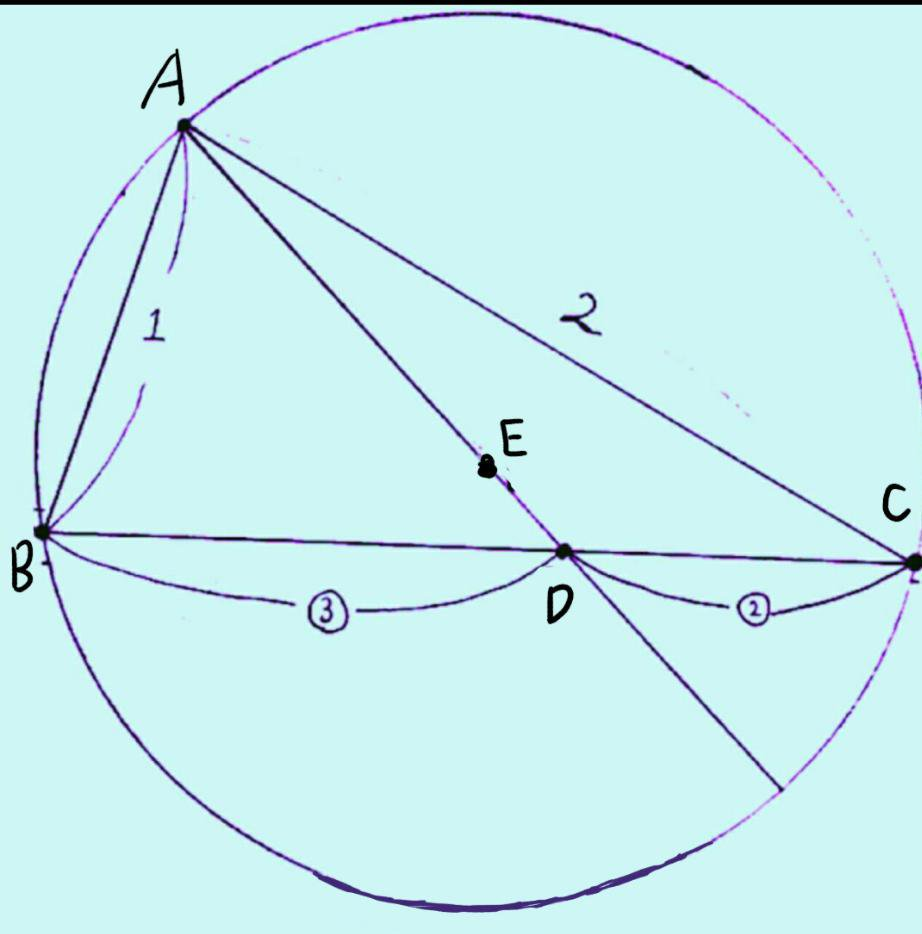
\includegraphics[bb=0 0 922 934,width=0.7\linewidth]{../problems/Q_070/Q_070.jpg}
 \end{center}
\end{thm}

線分AEに加えて、線分BE, CE (青線)は円Eの半径であるから、$\triangle\mr{ABE}$, $\triangle\mr{ACE}$は二等辺三角形となる。よって点Eから線分AB, ACへ垂線を下ろす(赤線)と、その足はそれぞれの線分の中点となる。この点をそれぞれM, Nとする。ここで$\angle\mr{AME}=\angle\mr{ANE}=90^\circ$。
\begin{figure}[H]
 \centering
 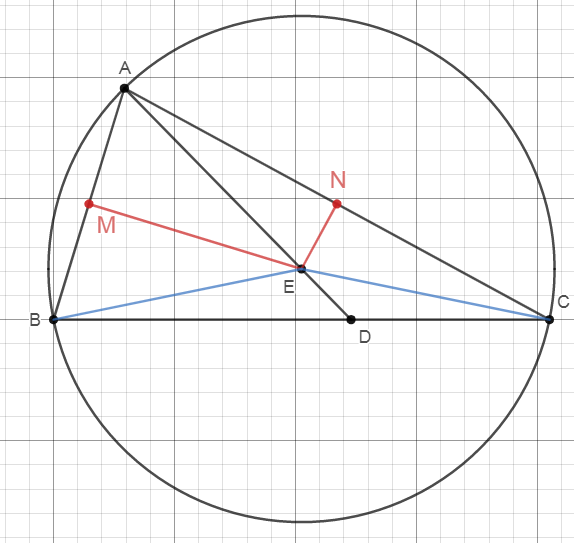
\includegraphics[width=0.7\linewidth]{../problems/Q_070/A_070-1.png}
\end{figure}
$\mr{BD}:\mr{BC}=3:2$より、$\triangle\mr{ABE}:\triangle\mr{ACE}=3:2$である。$\mr{AB}=1$, $\mr{AC}=2$であることから、$\mr{ME}:\mr{NE}=3:1$とわかる。よって$\mr{ME}=3x$, $\mr{NE}=x$とおけば、
\begin{align*}
 \left(\frac{1}{2}\right)^2+(3x)^2&=R^2 \\
 1^2+x^2&=R^2
\end{align*}
が得られる。ここで外接円の半径を$R$とした。 これらから、$R=\sqrt{\dfrac{35}{32}}$を得られた。

さて正弦定理によって、
\[ \frac{2}{\sin \mr{B}}=\frac{1}{\sin \mr{C}}=2R \quad\dou\quad \sin \mr{B}=\frac{1}{R} \,, \, \sin \mr{C}=\frac{1}{2R} \]
を得る。さて、このとき$\sin \mr{A}$は、
\begin{align*}
\sin \mr{A}&=\sin \left(180^\circ-(\mr{B}+\mr{C})\right)=\sin (\mr{B}+\mr{C}) \\
 &= \sin \mr{B} \cos \mr{C} + \cos \mr{B} \sin \mr{C}
\end{align*}
によって求められる。ここで、$\cos \mr{B}=\pm\sqrt{1-\dfrac{1}{R^2}}$, $\cos \mr{C}=\pm\sqrt{1-\dfrac{1}{4R^2}}$であり、符号は$\angle\mr{B}, \angle\mr{C}$が鋭角か鈍角かによって決定される。これを用いて$\sin \mr{A}$は、
\[ \sin \mr{A}=\frac{\pm\sqrt{4R^2-1}\pm\sqrt{R^2-1}}{2R^2} \]
と整理される。さて$0^\circ<\angle\mr{A}<180^\circ$であるから$\sin \mr{A}$は正でなければならない。よって$\angle\mr{C}$が鈍角であることは不適である。

求めるものは$\triangle\mr{ABC}$の面積で、
\begin{align*}
 \triangle\mr{ABC}&=\frac{1}{2}\mr{AB}\cdot \mr{AC} \cdot\sin \mr{A} \\
 &=\frac{1}{2}\times 1\times 2 \times \frac{\sqrt{4R^2-1}\pm\sqrt{R^2-1}}{2R^2} \\
 &=\frac{\sqrt{4R^2-1}\pm\sqrt{R^2-1}}{2R^2} \\
 &=\frac{2\sqrt{6}}{5} \,,\,\, \frac{2\sqrt{6}}{7}
\end{align*}
と求まった。なお前者は$\angle\mr{B}$が鋭角の場合、後者は鈍角の場合である。ちなみに$\angle\mr{B}$が鈍角の場合は、点Dは辺BCを$3:2$に外分し、図は以下のようになる。
\begin{figure}[H]
 \centering
 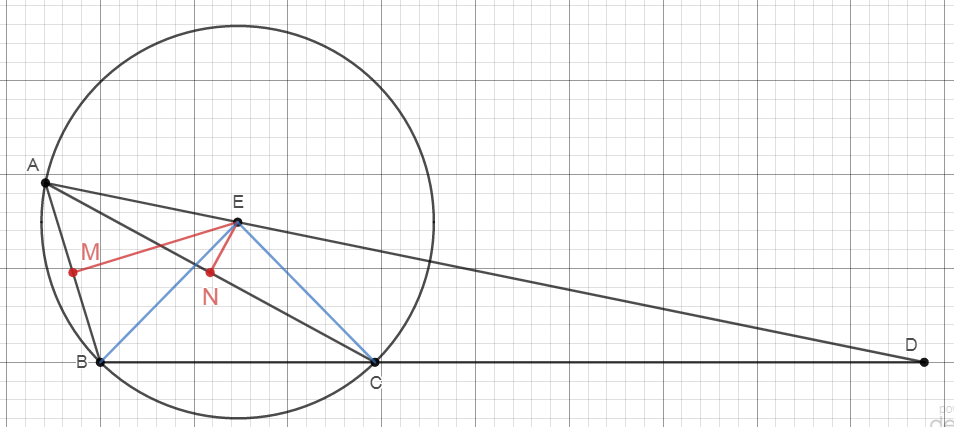
\includegraphics[width=0.9\linewidth]{../problems/Q_070/A_070-2.png}
\end{figure}



